%% Generated from runs/main_v1/analysis_v1/main_analysis.json (llm_judges.*.groups["platform=otf_r1|class=claude"].risk_coverage
%% and rule_judges["platform=otf_r1|class=claude"]). Do not edit numbers by hand; regenerate.
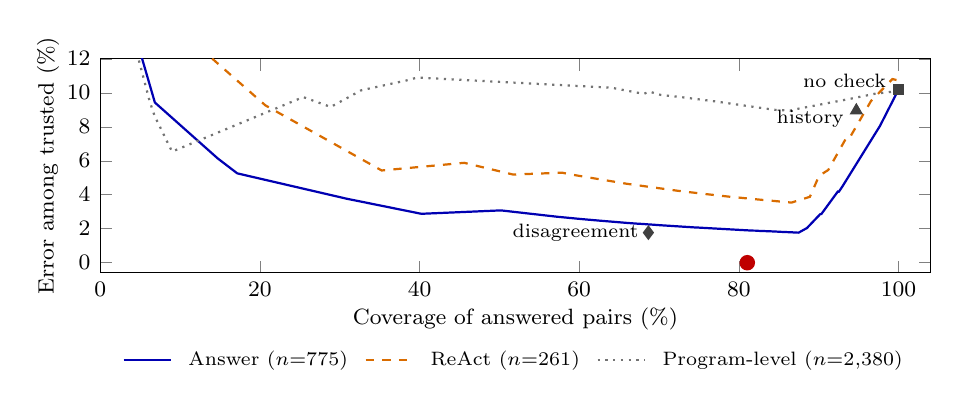
\begin{tikzpicture}
\begin{axis}[
  width=\columnwidth, height=4.3cm,
  xmin=0, xmax=104, ymin=-0.6, ymax=12,
  xlabel={Coverage of answered pairs (\%)}, ylabel={Error among trusted (\%)},
  xlabel style={font=\footnotesize, yshift=3pt}, ylabel style={font=\footnotesize, yshift=-4pt},
  tick label style={font=\footnotesize},
  xtick={0,20,40,60,80,100}, ytick={0,2,4,6,8,10,12},
  legend style={font=\scriptsize, at={(0.5,-0.31)}, anchor=north, draw=none, column sep=4pt},
  legend columns=3, legend cell align=left, clip=true,
]
\addplot[blue!70!black, thick, mark=none] coordinates {(0.39,33.33) (1.42,18.18) (6.84,9.43) (14.71,6.14) (17.16,5.26) (30.84,3.77) (40.00,2.90) (40.26,2.88) (50.19,3.08) (57.16,2.71) (60.26,2.57) (62.45,2.48) (62.97,2.46) (66.06,2.34) (67.23,2.30) (68.00,2.28) (68.26,2.27) (68.52,2.26) (68.90,2.25) (70.06,2.21) (74.71,2.07) (74.84,2.07) (81.29,1.90) (81.81,1.89) (82.06,1.89) (82.19,1.88) (83.87,1.85) (84.77,1.83) (85.55,1.81) (86.71,1.79) (86.84,1.78) (87.48,1.77) (88.52,2.04) (90.19,2.86) (90.32,2.86) (92.39,4.19) (92.52,4.18) (92.90,4.44) (97.68,8.06) (99.74,9.96) (100.00,10.19)};
\addlegendentry{Answer ($n{=}775$)}
\addplot[orange!85!black, thick, dashed, mark=none] coordinates {(1.15,66.67) (2.68,28.57) (8.81,13.04) (11.88,12.90) (20.69,9.26) (35.25,5.43) (45.59,5.88) (51.72,5.19) (57.85,5.30) (59.39,5.16) (59.77,5.13) (60.15,5.10) (65.90,4.65) (72.41,4.23) (75.86,4.04) (77.01,3.98) (79.31,3.86) (80.08,3.83) (81.99,3.74) (85.44,3.59) (86.59,3.54) (88.89,3.88) (90.04,5.11) (91.19,5.46) (93.49,7.38) (93.87,7.35) (96.55,9.52) (99.23,10.81) (100.00,10.73)};
\addlegendentry{ReAct ($n{=}261$)}
\addplot[black!55, thick, dotted, mark=none] coordinates {(0.46,36.36) (2.02,18.75) (2.31,16.36) (5.29,11.11) (6.18,9.52) (6.60,8.92) (6.81,8.64) (8.99,6.54) (25.42,9.75) (28.87,9.17) (32.69,10.15) (38.36,10.73) (39.71,10.90) (64.03,10.30) (68.07,9.94) (68.82,10.07) (69.58,9.96) (70.13,9.89) (70.17,9.88) (72.90,9.74) (76.97,9.50) (84.45,9.00) (85.71,8.97) (86.39,8.95) (87.06,9.03) (93.53,9.61) (97.10,9.95) (99.29,10.07) (100.00,10.21)};
\addlegendentry{Program-level ($n{=}2{,}380$)}
\addplot[only marks, forget plot, mark=square*, mark size=1.8pt, black!75] coordinates {(100.00,10.21)};
\node[font=\scriptsize, left, xshift=-1pt, yshift=3pt] at (axis cs:100.00,10.21) {no check};
\addplot[only marks, forget plot, mark=triangle*, mark size=2.4pt, black!75] coordinates {(94.71,8.96)};
\node[font=\scriptsize, left, xshift=-1pt, yshift=-3pt] at (axis cs:94.71,8.96) {history};
\addplot[only marks, forget plot, mark=diamond*, mark size=2.4pt, black!75] coordinates {(68.66,1.77)};
\node[font=\scriptsize, left] at (axis cs:68.66,1.77) {disagreement};
\addplot[only marks, forget plot, mark=*, mark size=2.6pt, red!75!black] coordinates {(81.05,0.00)};
\node[font=\scriptsize, above, yshift=1pt] at (axis cs:81.05,0.00) {\gate};
\end{axis}
\end{tikzpicture}
